\chapter{Σχεδίαση και αρχιτεκτονική λογισμικού}
\label{ch:architecture}
% Στην ενότητα αυτή θα περιγραφούν τα βασικά συστατικά του συστήματος καθώς και οι σχέσεις που τα συνδέουν μεταξύ τους.
Στη ενότητα αυτή, θα περιγραφούν οι βασικές αρχές λειτουργίας του εργαλείου, το οποίο μπορεί κάποιος να βρει 
στο \href{https://github.com/tasakos-dev/Design-pattern-builder}{\color{blue}\underline{github}}. 
πρόκειται για ένα εργαλείο το οποίο αποτελεί επέκταση του Eclipse και έχει σχεδιαστεί σε γλώσσα java. 
αποτελείται από δύο τμήματα, το ένα κομμάτι αποτελείται από τον πηγαίο κώδικα του εργαλείου. Το άλλο τμήμα του εργαλείου είναι 
ένα αρχείο στο οποίο περιγράφουμε με δομημένο τρόπο κάθε σχεδιαστικό μοτίβο των GoF \cite{GoF}. Στην ουσία, δημιουργήσαμε ένα εργαλείο, 
το οποίο έχει την δυνατότητα να παράξει πηγαίο κώδικα java, διαβάζοντας ένα αρχείο στο οποίο υπάρχουν οι περιγραφές 
κάθε κλάσης και διεπαφής. Καθώς θέλαμε να υπάρχει η δυνατότητα δομημένης περιγραφής για την κάθε κατηγορία και κάθε μοτίβο, επιλέξαμε 
να χρησιμοποιήσουμε την γλώσσα περιγραφής xml. Για την περιγραφή της δομής κάθε μοτίβου, 
δημιουργήσαμε ένα αρχείο xml, το οποίο φαίνεται στην εικόνα \ref{fig:xsd}, όπως και ένα παράδειγμα ενός μοτίβου \ref{code:xml}, 
καθώς μπορεί κάποιος πολύ εύκολα να επεκτείνει τα διαθέσιμα μοτίβα, απλώς τροποποιώντας το αρχείο αυτό, 
χωρίς να κάνει αλλαγές στον κώδικα, καθώς και μεταγλώττιση του κώδικα και ελέγχους. 
Το εργαλείο διαβάζει το αρχείο xml, δημιουργεί εσωτερικά κατάλληλες δομές, ώστε στη συνέχεια, η γραφική διεπαφή 
να μπορεί να διαχειριστεί τις κλάσεις και διεπαφές του μοτίβου, όπως και τις μεθόδους και πεδία. Προσφέροντας την δυνατότητα στον χρήστη, 
να αλληλεπιδρά με τα διάφορα μοτίβα. Καθώς ο προγραμματιστής αλληλεπιδρά με την γραφική διεπαφή, 
το σύστημα ενημερώνει συνεχώς τις δομές αυτές, ώστε όταν ο προγραμματιστής έχει παραμετροποιήσει κατάλληλα το μοτίβο, 
το σύστημα να είναι σε θέση να εξάγει τα πηγαία αρχεία, ώστε το τελικό αποτέλεσμα να ανταποκρίνεται στις απαιτήσεις του προγραμματιστή.
\newline \newline
Όταν ο χρήστης ανοίξει τον οδηγό, δηλαδή την γραφική διεπαφή του εργαλείου, το σύστημα διαβάζει το αρχείο xml 
και εμφανίζει στην γραφική διεπαφή τις διαθέσιμες κατηγορίες, αφού ο προγραμματιστής διαλέξει κάποια κατηγορία, 
τότε εμφανίζει στον προγραμματιστή τα διαθέσιμα μοτίβα αυτής της κατηγορίας. Στη συνέχεια, 
ο προγραμματιστής μπορεί να προσθέσει νέα κλάση, εάν αυτό επιτρέπεται, να τροποποιήσει τις κλάσεις, δηλαδή να αλλάξει το όνομα τους, 
να επιλέξει κάποια διεπαφή για να υλοποιήσει, εάν είναι νέα κλάση και όχι κλάση του μοτίβου, 
τέλος να επεξεργαστεί τα πεδία και τις μεθόδους, καθώς και να προσθέσει νέα πεδία και μεθόδους. Αφού ο προγραμματιστής κάνει τις αλλαγές που επιθυμεί και πατήσει
finish, τότε το σύστημα θα ενημερώσει κατάλληλα τις δομές,  Αντίστοιχα, ο προγραμματιστής μπορεί να τροποποιήσει 
και τις διεπαφές του μοτίβου και το σύστημα με ανάλογο τρόπο ενημερώνει τις δομές του πεδίου εφαρμογής. \newline \newline

% To υποσύστημα του εργαλείου το οποίο είναι υπεύθυνο για διαβάζει το αρχείο xml, δημιουργεί πίνακες από Strings με τις απαιτούμενες πληροφορίες,  
% δηλαδή εάν ζητούνται οι κλάσεις ενός μοτίβου θα δημιουργηθεί ένας πίνακας με τα ονόματα των κλάσεων, 
% εάν ζητούνται οι μέθοδοι μίας κλάσης θα δημιουργηθεί ένας πίνακας ο οποίος περιέχει για κάθε μέθοδο έναν 
% πίνακα με την ορατότητα της μεθόδου, τον επιστρεφόμενο τύπο της μεθόδου και το όνομα της. Αντίστοιχα δημιουργούνται πίνακες 
% για τις διεπαφές και τα πεδία. Στη συνέχεια, ο controller χρησιμοποιεί τον parser για να αντλήσει τα ωμά δεδομένα 
% και να τα μετασχηματίσει σε κατάλληλες δομές ώστε να μπορεί η γραφική διεπαφή να τις διαχειριστεί, οι δομές αυτές είναι 
% οι κλάσεις που αναπαριστούν το πεδίο της εφαρμογής μας, δηλαδή οι κλάσεις του πακέτου model. \newline \newline
% % Όταν ο χρήστης ανοίξει τον οδηγό, δηλαδή την γραφική διεπαφή του εργαλείου, το σύστημα διαβάζει δια μέσου του FileParser το αρχείο xml 
% % και με την βοήθεια του controller, εμφανίζει στην γραφική διεπαφή τις διαθέσιμες κατηγορίες, αφού ο προγραμματιστής διαλέξει κάποια κατηγορία, 
% % τότε το σύστημα με αντίστοιχο τρόπο εμφανίζει στον προγραμματιστή τα διαθέσιμα μοτίβα αυτής της κατηγορίας. Στη συνέχεια, 
% % ο προγραμματιστής μπορεί να προσθέσει νέα κλάση, εάν αυτό επιτρέπεται, να τροποποιήσει τις κλάσεις, δηλαδή να αλλάξει το όνομα τους, 
% % να επιλέξει κάποια διεπαφή για να υλοποιήσει, εάν είναι νέα κλάση και όχι κλάση του μοτίβου, 
% τέλος να επεξεργαστεί τα πεδία και τις μεθόδους, καθώς και να προσθέσει νέα πεδία και μεθόδους. Αφού ο προγραμματιστής κάνει τις αλλαγές που επιθυμεί και πατήσει
% finish, τότε το σύστημα θα ενημερώσει κατάλληλα τα αντικείμενα που ανήκουν στο πακέτο model, χρησιμοποιώντας μεθόδους του υποσυστήματος controller και 
% πιο συγκεκριμένα της κλάσης PatternManager, ώστε να ενημερωθούν σωστά τα ονόματα. Αντίστοιχα, ο προγραμματιστής μπορεί να τροποποιήσει 
% και τις διεπαφές του μοτίβου και το σύστημα με ανάλογο τρόπο ενημερώνει τις δομές του πεδίου εφαρμογής. \newline \newline
Το υποσύστημα της γραφικής διεπαφής, είναι πλήρως εξαρτημένο από το API του Eclipse, καθώς είναι 
βασισμένο στην κλάση Wizard που προσφέρει το Eclipse και η οποία παρέχει τη λειτουργικότητα για τη δημιουργία 
προσαρμοσμένων οδηγών. Ο οδηγός είναι μια σειρά σελίδων που καθοδηγούν τον χρήστη σε μια σύνθετη εργασία. 
Τα κουμπιά Πίσω και Επόμενο επιτρέπουν στο χρήστη να μετακινείται προς τα εμπρός και προς τα πίσω στις σελίδες. 
Συνήθως, κάθε σελίδα συλλέγει μια πληροφορία\anotelia \  Όταν ο χρήστης κάνει κλικ στο κουμπί Τέλος, οι πληροφορίες χρησιμοποιούνται 
για την εκτέλεση μιας εργασίας. Ανά πάσα στιγμή πριν από το κλικ στο κουμπί Finish, ο χρήστης μπορεί να ακυρώσει την εργασία, 
γεγονός που θα πρέπει να αναιρέσει τυχόν παρενέργειες των βημάτων που έχουν ολοκληρωθεί μέχρι στιγμής. Τέλος, ένα τμήμα 
του εργαλείου, το οποίο είναι υπεύθυνο για την δημιουργία των πηγαίων αρχείων, εξαρτάται από το API του Eclipse, καθώς χρησιμοποιεί, 
την κλάση PackageFragment, η οποία παρέχει διάφορες λειτουργίες που είναι απαραίτητες για την σωστή εξαγωγή των μοτίβων, 
όπως ο εντοπισμός του classpath για την προσθήκη των annotations, την εύρεση της τοποθεσίας όπου θα δημιουργηθούν τα πηγαία αρχεία 
καθώς και την ίδια την δημιουργία ενός πηγαίου αρχείου.

\begin{figure}[H]
    \centering
    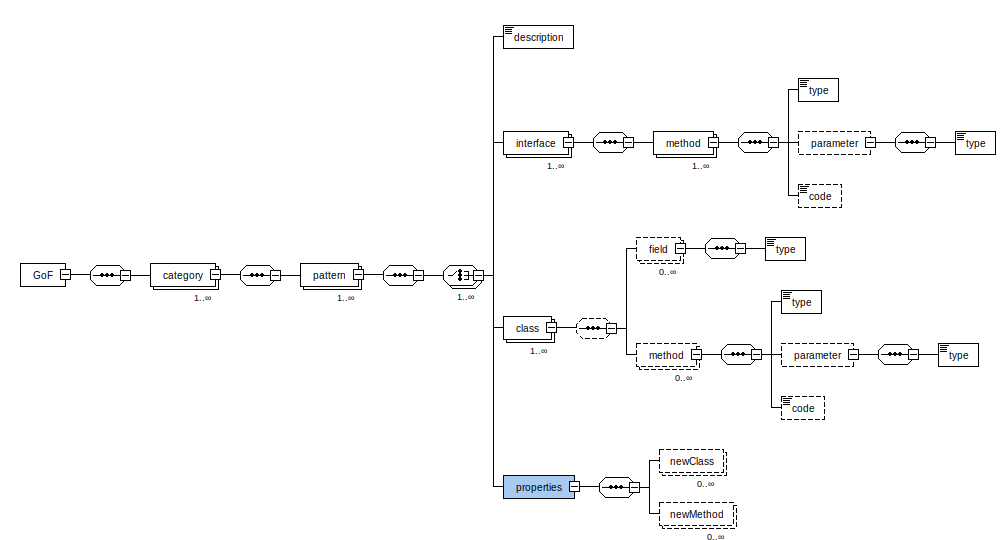
\includegraphics[width=1.0\textwidth]{Figures/xsd_diagram.png}
    \caption{Σχήμα αρχείου xml.}
    \label{fig:xsd}
\end{figure}
\newpage
\begin{lstlisting}[label=code:xml, caption=Περιγραφή μοτίβου Singleton.]
<pattern id="Singleton">
    <description>
        Ensure a class only has one instance, 
        and provide a global point of access to it.
    </description>
    <class id="Singleton" annotation="Singleton">
        <field id="instance" isStatic="true">
            <type>Singleton</type>
        </field>
        <method id="Singleton" visibility="private">
            <type></type>
        </method>
        <method id="getInstance" isStatic="true">
            <type>Object</type>
            <code>
                if (instance == null) {
                    instance = new Singleton();
                }
                return instance;
            </code>
        </method>
    </class>
</pattern>
\end{lstlisting}
\section{Αρχιτεκτονική}
\label{sec:packages}
\begin{figure}[H]
    \centering
    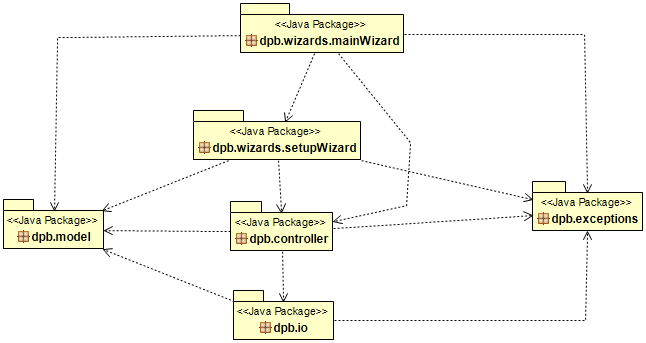
\includegraphics[width=1.0\textwidth]{Figures/packages.png}
    \caption{Διάγραμμα UML Πακέτων συστήματος.}
    \label{fig:packageUML}
\end{figure}
% \begin{figure}[H]
%     \centering
%     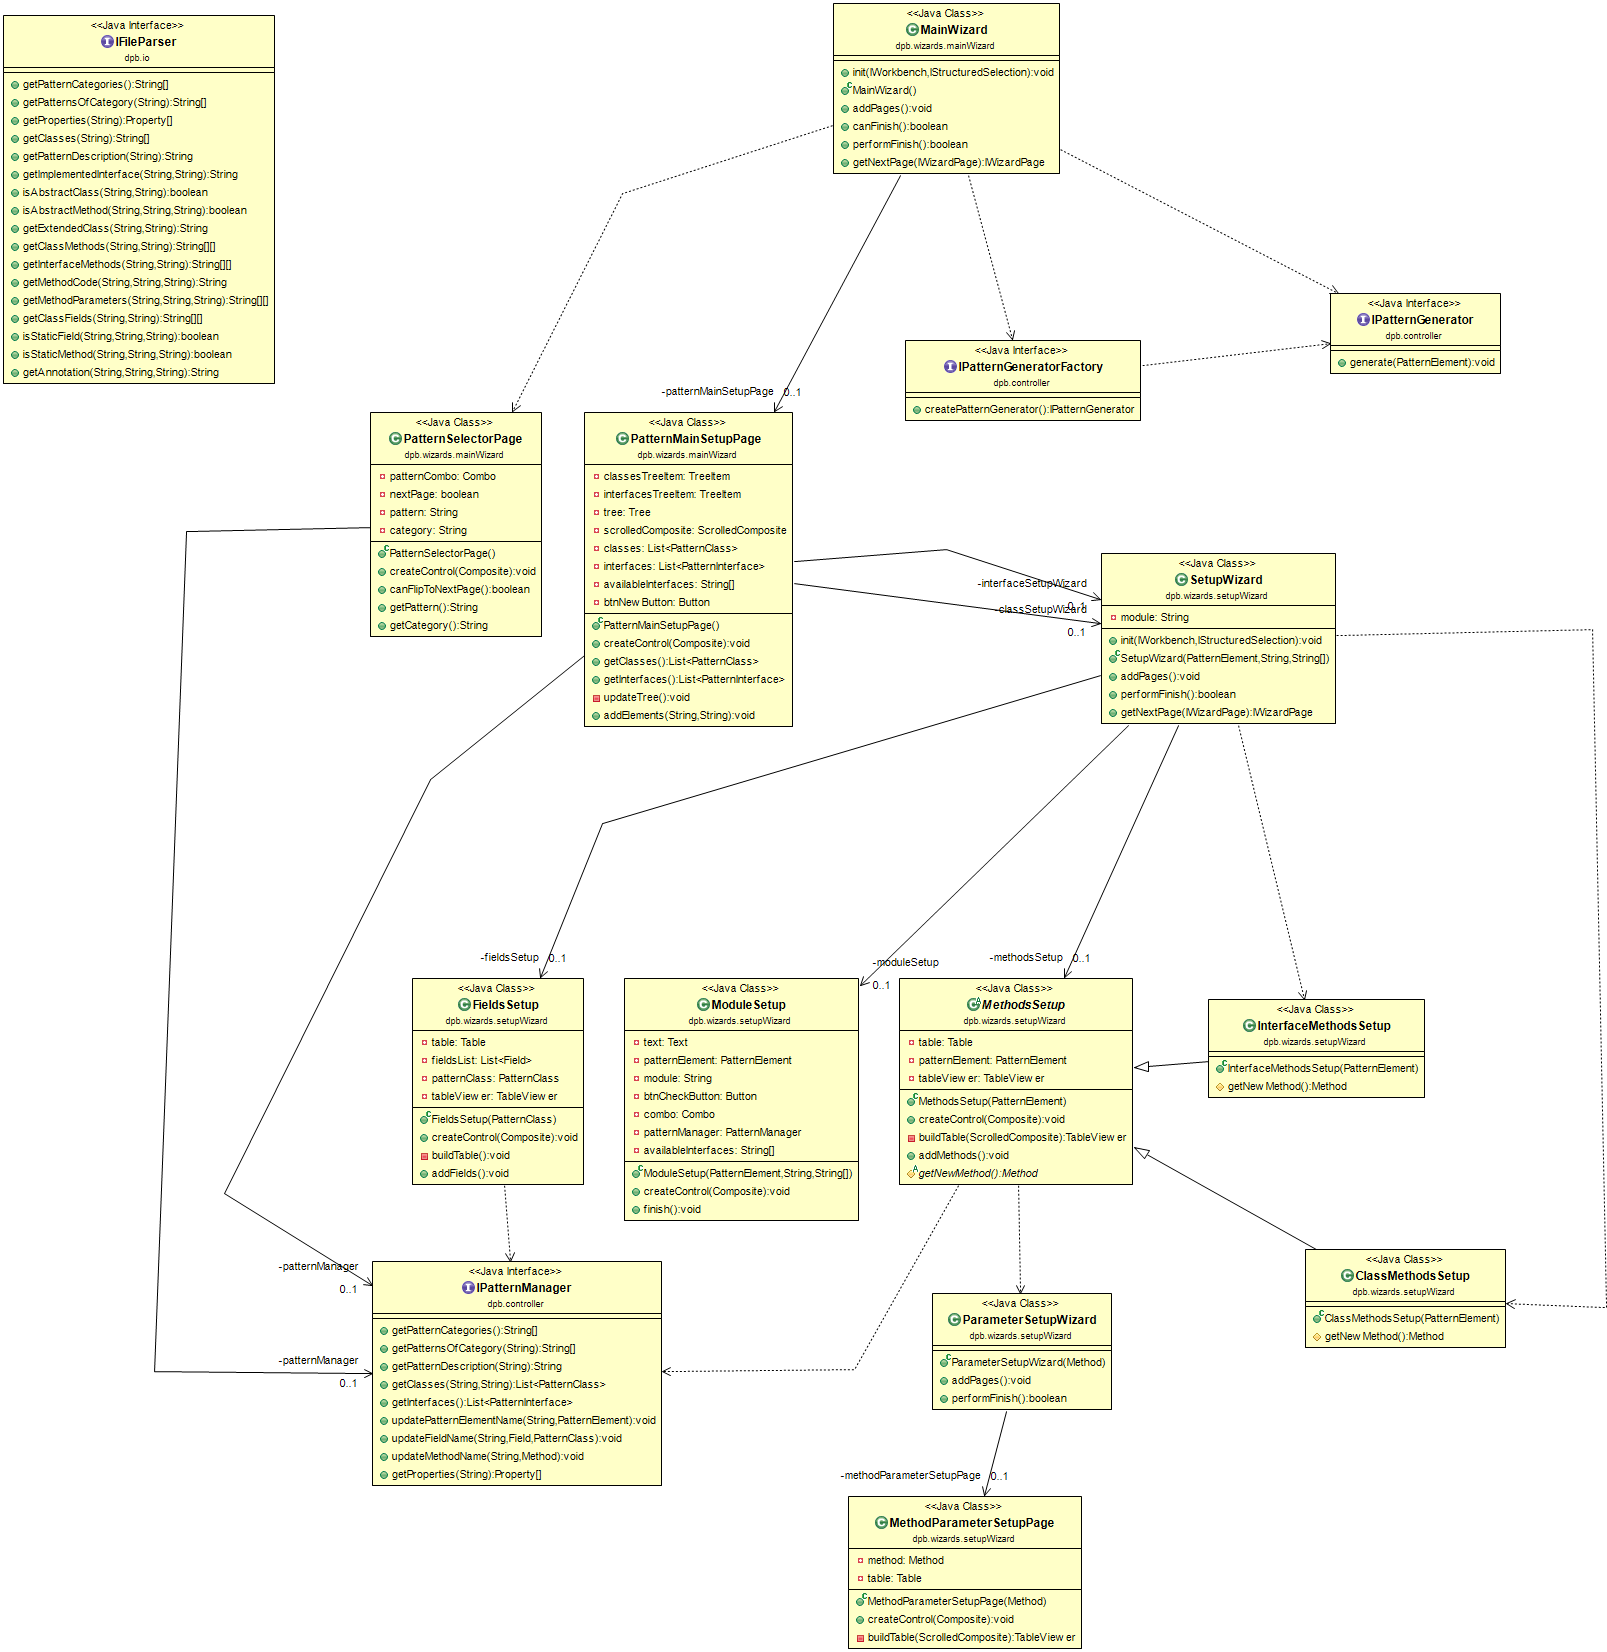
\includegraphics[width=1.0\textwidth]{Figures/system.png}
%     \caption{Διάγραμμα UML κλάσεων \& διεπαφών συστήματος.}
%     \label{fig:systemUML}
% \end{figure}

Το λογισμικό αποτελείται από τα παρακάτω πακέτα,
\begin{itemize}
    \item dpb.wizards.mainWizard, σε αυτό το πακέτο, περιέχονται οι κλάσεις που αφορούν το γραφικό περιβάλλον του εργαλείου,
     πιο συγκεκριμένα, οι κλάσεις αυτού του πακέτου έχουν να κάνουν με την επιλογή του μοτίβου και την διαχείριση των κλάσεων και διεπαφών του 
     επιλεγμένου μοτίβου.
    \item dpb.wizards.setupWizards, σε αυτό το πακέτο, υπάρχουν οι κλάσεις που έχουν σχέση με την γραφική διεπαφή και την τροποποίηση των κλάσεων και διεπαφών, 
    όπως και των μεθόδων και πεδίων.
    \item dpb.controller, αποτελεί το πακέτο μέσω του οποίου η γραφική διεπαφή επικοινωνεί με το back-end. Χρησιμοποιεί τις λειτουργίες που παρέχει το back-end, 
    ώστε να  μετασχηματίζει τα ακατέργαστα δεδομένα των μοτίβων που παίρνει από το υποσύστημα io σε αντικείμενα κλάσεων που παρέχει το πακέτο model.
    \item dpb.io, αποτελεί το κομμάτι του συστήματος το οποίο χαρακτηρίζεται ως back-end.
     και είναι υπεύθυνο για το διάβασμα του αρχείου xml στο οποίο περιγράφονται τα μοτίβα. 
     Παρέχει λειτουργίες για την εισαγωγή των μοτίβων στο σύστημα.
    \item dpb.model, Το πακέτο αυτό, περιέχει τις κλάσεις οι οποίες αναπαριστούν τα αντικείμενα του πεδίου του προβλήματος.
    \item dpb.exceptions, Τέλος, στο πακέτο αυτό υπάρχουν κάποιες κλάσεις οι οποίες αναπαριστούν εξαιρέσεις 
        οι οποίες είναι κάποια γεγονότα που συμβαίνουν κατά την εκτέλεση του εργαλείου και διακόπτουν την κανονική ροή του προγράμματος.
\end{itemize}
To υποσύστημα του εργαλείου το οποίο είναι υπεύθυνο για διαβάζει το αρχείο xml, το υποσύστημα io, 
δημιουργεί πίνακες από Strings με τις απαιτούμενες πληροφορίες, δηλαδή εάν ζητούνται οι κλάσεις ενός μοτίβου 
θα δημιουργηθεί ένας πίνακας με τα ονόματα των κλάσεων, εάν ζητούνται οι μέθοδοι μίας κλάσης θα δημιουργηθεί ένας πίνακας 
ο οποίος περιέχει για κάθε μέθοδο έναν πίνακα με την ορατότητα της μεθόδου, τον επιστρεφόμενο τύπο της μεθόδου και το όνομα της. 
Αντίστοιχα δημιουργούνται πίνακες για τις διεπαφές και τα πεδία. Στη συνέχεια, το υποσύστημα του controller, 
χρησιμοποιεί τον parser για να αντλήσει τα ωμά δεδομένα και να τα μετασχηματίσει σε κατάλληλες δομές ώστε να μπορεί 
η γραφική διεπαφή να τις διαχειριστεί, οι δομές αυτές είναι οι κλάσεις που αναπαριστούν το πεδίο της εφαρμογής μας, 
δηλαδή οι κλάσεις του πακέτου model. 
% \newline \newline
% Όταν ο χρήστης ανοίξει τον οδηγό, δηλαδή την γραφική διεπαφή του εργαλείου, το σύστημα διαβάζει δια μέσου του FileParser το αρχείο xml 
% και με την βοήθεια του controller, εμφανίζει στην γραφική διεπαφή τις διαθέσιμες κατηγορίες, αφού ο προγραμματιστής διαλέξει κάποια κατηγορία, 
% τότε το σύστημα με αντίστοιχο τρόπο εμφανίζει στον προγραμματιστή τα διαθέσιμα μοτίβα αυτής της κατηγορίας. Στη συνέχεια, 
% ο προγραμματιστής μπορεί να προσθέσει νέα κλάση, εάν αυτό επιτρέπεται, να τροποποιήσει τις κλάσεις, δηλαδή να αλλάξει το όνομα τους, 
% να επιλέξει κάποια διεπαφή για να υλοποιήσει, εάν είναι νέα κλάση και όχι κλάση του μοτίβου, 
% τέλος να επεξεργαστεί τα πεδία και τις μεθόδους, καθώς και να προσθέσει νέα πεδία και μεθόδους. Αφού ο προγραμματιστής κάνει τις αλλαγές που επιθυμεί και πατήσει
% finish, τότε το σύστημα θα ενημερώσει κατάλληλα τα αντικείμενα που ανήκουν στο πακέτο model, χρησιμοποιώντας μεθόδους του υποσυστήματος controller και 
% πιο συγκεκριμένα της κλάσης PatternManager, ώστε να ενημερωθούν σωστά τα ονόματα. Αντίστοιχα, ο προγραμματιστής μπορεί να τροποποιήσει 
% και τις διεπαφές του μοτίβου και το σύστημα με ανάλογο τρόπο ενημερώνει τις δομές του πεδίου εφαρμογής.

% \newpage
% \section{Κλάσεις συστήματος}
% \label{sec:classes}
% \subsection{Ανάλυση κλάσεων}
% \label{subsec:classAnalysis}
% Παρακάτω, θα αναλύσουμε κάποιες βασικές κλάσεις του συστήματος,
% \begin{itemize}
%     \item PatternClass, η κλάση αυτή ανήκει στο πακέτο model και μοντελοποιεί μία κλάση του μοτίβου
%     \item PatternInterface, η κλάση αυτή ανήκει στο πακέτο model και μοντελοποιεί μία διεπαφή του μοτίβου
%     \item Method, η κλάση αυτή ανήκει στο πακέτο model και μοντελοποιεί μία μέθοδο που ανήκει σε κλάση ή διεπαφή του μοτίβου
%     \item Field, η κλάση αυτή ανήκει στο πακέτο model και μοντελοποιεί ένα πεδίο που ανήκει σε κλάση του μοτίβου
%     \item FileParser, είναι η βασική κλάση του υποσυστήματος io, είναι υπεύθυνη για το διάβασμα του αρχείου όπου περιγράφονται
%     τα μοτίβα και η βασική της δουλειά είναι να διαβάζει το αρχείο xml. Υποστηρίζει λειτουργίες όπως η ανάκτηση 
%     των κατηγοριών και των μοτίβων κάθε κατηγορίας, η ανάκτηση των κλάσεων και διεπαφών ενός μοτίβου, 
%     η ανάκτηση των annotations κάθε στοιχείου για κάποιο μοτίβο, όπως και οι ιδιότητες ενός μοτίβου 
%     οι οποίες είναι εάν επιτρέπεται η εισαγωγή νέας κλάσης, τέλος υποστηρίζει την ανάκτηση μεθόδων και πεδίων.
%     \item PatternManager, Μέσω της κλάσης αυτής παρέχεται η δυνατότητα στην γραφική διεπαφή του συστήματος 
%     να αντλεί οτιδήποτε χρειάζεται από το υποσύστημα io
%     \item PatternGenerator, Περιλαμβάνει την λειτουργία δημιουργίας των πηγαίων αρχείων στο πακέτο του έργου που έχει επιλέξει 
%     ο προγραμματιστής ή στο προεπιλεγμένο πακέτο, εάν δεν έχει επιλέξει κάποιο πακέτο, τα οποία περιέχουν 
%     τις κλάσεις του μοτίβου με τις μεθόδους και τα πεδία, όπως τα παραμετροποίησε ο προγραμματιστής, καθώς και τις διεπαφές. 
%     Επίσης προσθέτει στο classpath του έργου του προγραμματιστή το πακέτο που περιέχει τα annotations 
%     ώστε να είναι διαθέσιμα στον προγραμματιστή.
     
% \end{itemize}

\section{dpb.wizards.mainWizard}
\label{sec:dpb.wizards.mainWizard}
\begin{figure}[H]
    \centering
    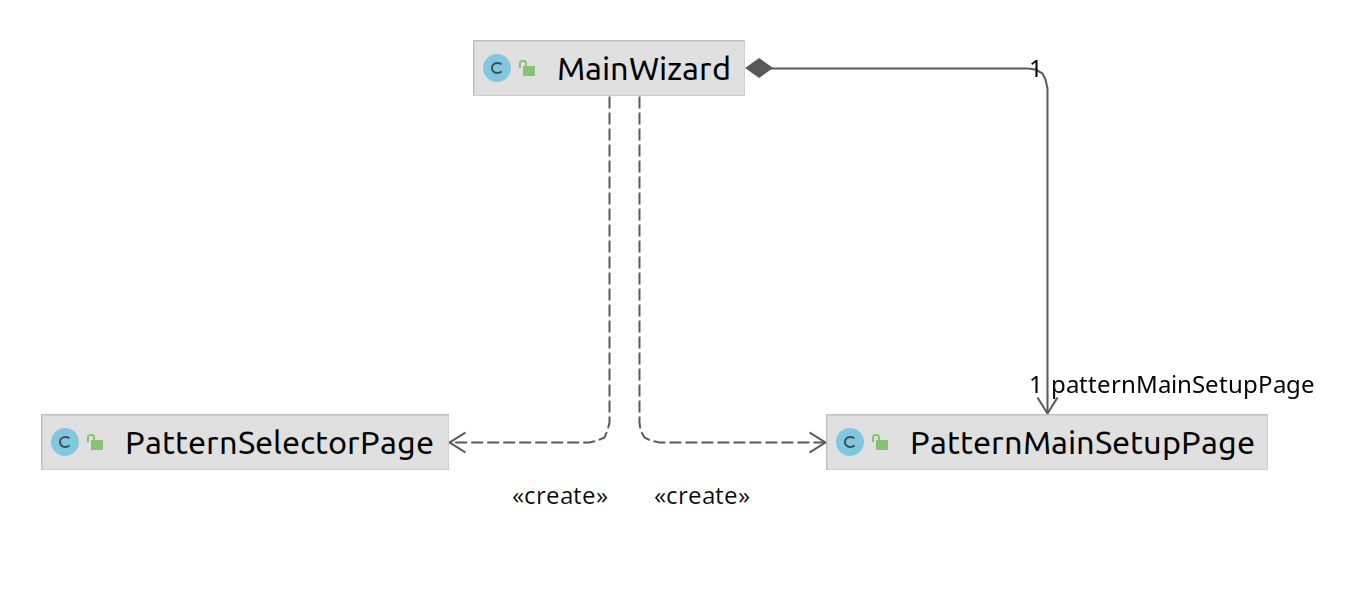
\includegraphics[width=1.0\textwidth]{Figures/mainWizard.png}
    \caption{Διάγραμμα UML Πακέτου mainWizard.}
    \label{fig:mainWizardUML}
\end{figure}
Το υποσύστημα αυτό, έχει να κάνει με τον κύριο οδηγό του εργαλείου, ο οποίος αποτελείται από δύο σελίδες. Η πρώτη σελίδα, 
δίνει στον προγραμματιστή την δυνατότητα να επιλέξει κατηγορία και μοτίβο. Στην δεύτερη σελίδα ο προγραμματιστής μπορεί να περιηγηθεί 
ανάμεσα στις διαθέσιμες κλάσεις και διεπαφές, καθώς και να προσθέσει κάποια καινούργια κλάση, 
εάν αυτό είναι δυνατό από τους περιορισμούς που ορίζονται στην περιγραφή των μοτίβων, 
όπως και να επεξεργαστεί τις κλάσεις και τις διεπαφές. η κλάση που υλοποιεί τον οδηγό, είναι η κλάση MainWizard, επεκτείνει την κλάση Wizard που παρέχει 
το Eclipse και υλοποιεί την διεπαφή INewWizard, η αρμοδιότητα της είναι να προσθέτει τις σελίδες του οδηγού αυτού, και να χειρίζεται 
το γεγονός κατά το οποίο προγραμματιστής έχει τελειώσει με την ρύθμιση του μοτίβου και κάνει κλικ στο κουμπί Τέλος, τότε καλείται η μέθοδος generate της κλάσης PatternGenerator,
για κάθε κλάση και διεπαφή του μοτίβου, η οποία θα αναλυθεί στην ενότητα \ref{sec:dpb.controller} και είναι υπεύθυνη για την παραγωγή των πηγαίων αρχείων.
Η κλάση PatternSelectonPage η οποία επεκτείνει την κλάση WizardPage και υλοποιεί την διεπαφή IWizardPage, 
είναι η πρώτη σελίδα του κύριου μας οδηγού, αυτό που κάνει είναι να χρησιμοποιεί την κλάση PatternManager, η οποία 
θα αναλυθεί στην ενότητα \ref{sec:dpb.controller}, ώστε να αντλήσει τις κατηγορίες των μοτίβων και να τις εμφανίσει σε μία λίστα, 
όταν επιλεχθεί μία κατηγορία από τον προγραμματιστή τότε ενεργοποιεί μία δεύτερη λίστα στην οποία προσθέτει 
τα μοτίβα αυτής της κατηγορίας. Τέλος η τελευταία κλάση του πακέτου αυτού είναι η κλάση PatternMainSetupPage 
η οποία και αυτή υλοποιεί και επεκτείνει αντίστοιχα τα IWizardPage και WizardPage, κύρια της δουλειά είναι η εμφάνιση των κλάσεων και διεπαφών 
του επιλεγμένου μοτίβου τα οποία αντλεί και αυτή με την χρήση του υποσυστήματος controller, και παρέχει κουμπιά για την προσθήκη νέας κλάσης, καθώς και 
την επεξεργασία των κλάσεων και διεπαφών, όταν ο χρήστης κάνει κλικ σε κάποιο κουμπί επεξεργασίας, τότε δημιουργείται 
ο δεύτερος οδηγός της γραφικής διεπαφής ο οποίος θα αναλυθεί στην ενότητα \ref{sec:dpb.wizards.setupWizards}.\newpage
\section{dpb.wizards.setupWizards}
\label{sec:dpb.wizards.setupWizards}
\begin{figure}[H]
    \centering
    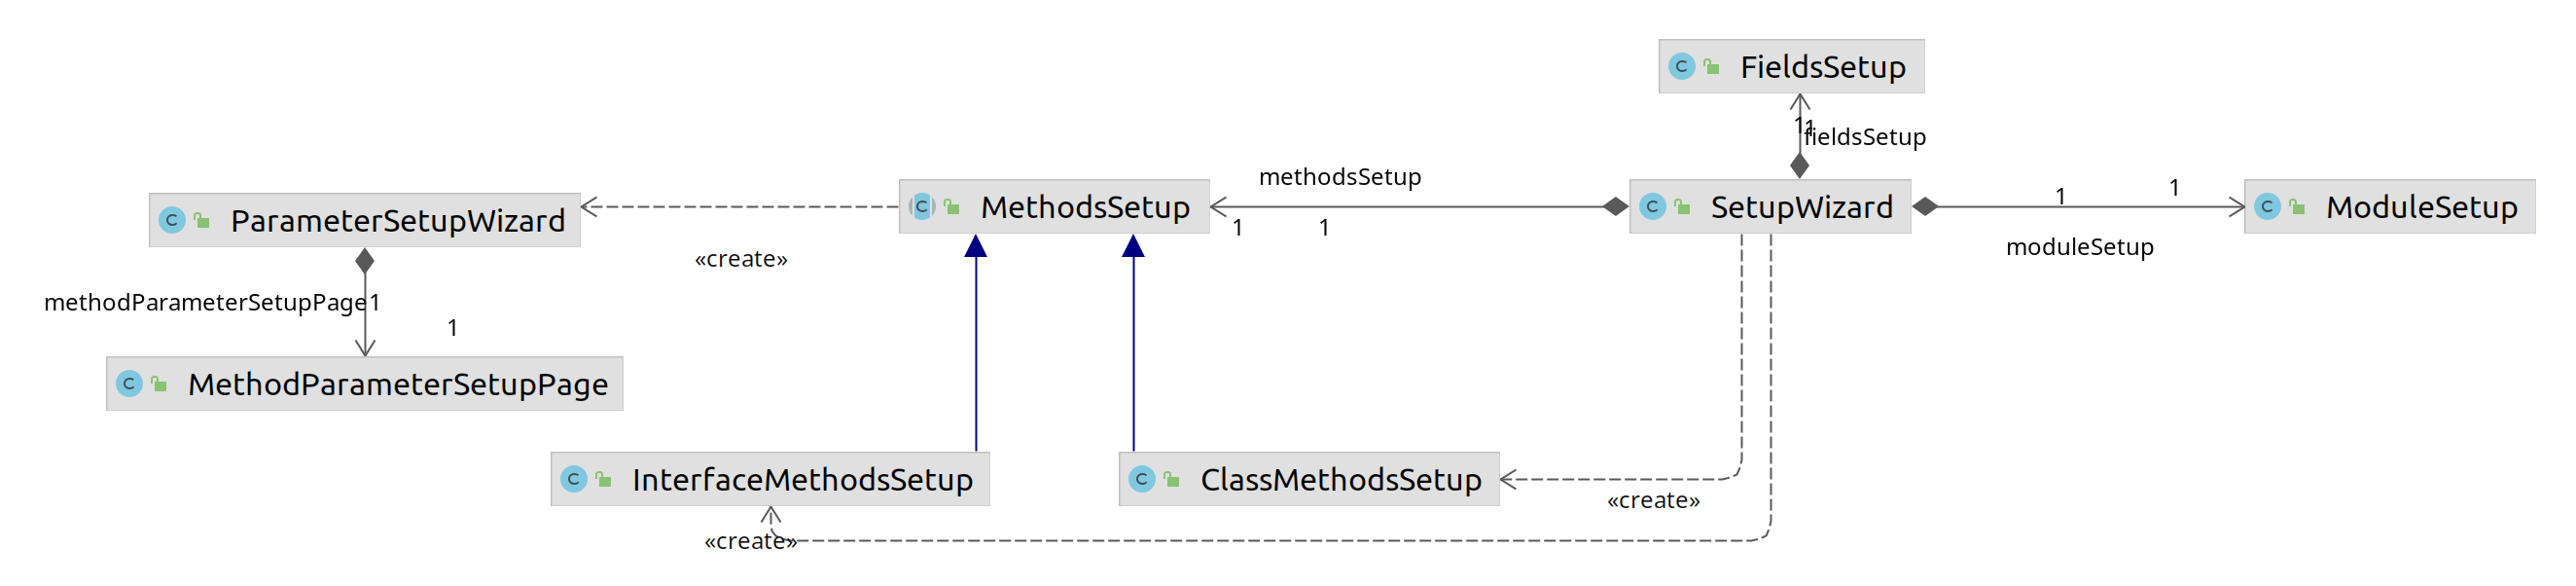
\includegraphics[width=1.0\textwidth]{Figures/setupWizard.png}
    \caption{Διάγραμμα UML Πακέτου setupWizards.}
    \label{fig:setupWizardUML}
\end{figure}
Το υποσύστημα αυτό, αποτελείται από δύο οδηγούς, ο πρώτος οδηγός είναι υπεύθυνος για την ρύθμιση των ονομάτων κλάσεων και διεπαφών, 
για την επιλογή κάποιας διεπαφής που θα υλοποιεί μία νέα κλάση, καθώς και για την ρύθμιση των πεδίων και μεθόδων. 
Η κλάση που υλοποιεί τον οδηγό αυτόν, είναι η κλάση SetupWizard, προσθέτει τις κατάλληλες σελίδες στον οδηγό, δηλαδή εάν ο προγραμματιστής 
θέλει να επεξεργαστεί μία κλάση τότε θα προσθέσει τρεις σελίδες, αλλιώς εάν επεξεργάζεται διεπαφή δύο σελίδες. 
Η τελευταία σελίδα είναι παρόμοια και για τις δύο περιπτώσεις, αφορά την επεξεργασία μεθόδων και υλοποιείται από την κλάση MethodsSetup,
Εμφανίζει στον προγραμματιστή όλες τις μεθόδους που ανήκουν στην κλάση ή διεπαφή που επεξεργάζεται αυτήν την στιγμή, 
ο προγραμματιστής έχει την δυνατότητα να αλλάξει το όνομα, την ορατότητα, καθώς και τον επιστρεφόμενο τύπο κάθε μεθόδου, 
επίσης έχει την δυνατότητα να προσθέσει ή διαγράψει κάποια μέθοδο, ακόμα μπορεί να επεξεργαστεί τις παραμέτρους κάποιας μεθόδου, 
για την λειτουργία αυτή, αναπτύχθηκε ακόμα ένας οδηγός ο οποίος υλοποιείται από την κλάση ParameterSetupWizard, 
έχει μία σελίδα, την MethodParameterSetup, η οποία εμφανίζει μία λίστα με τις παραμέτρους της επιλεγμένης μεθόδου και ο προγραμματιστής, 
έχει την δυνατότητα να αλλάξει το όνομα και τύπο κάθε παραμέτρου, καθώς και να προσθέσει ή διαγράψει κάποια παράμετρο. 
Μόλις ο χρήστης αλλάξει κάποια παράμετρο αυτομάτως ενημερώνεται και το αντικείμενο τύπου Parameter. 
Αντίστοιχα μόλις ο προγραμματιστής παραμετροποιεί κάποια μέθοδο τότε αυτομάτως ενημερώνεται και η δομή Method που αντιπροσωπεύει την μέθοδο αυτήν.
Ακόμα, και η πρώτη σελίδα είναι κοινή, υλοποιείται από την κλάση ModuleSetup, αλλά εάν πρόκειται για κλάση τότε περιέχει 
% ένα κουμπί που ελέγχει εάν η κλάση θα είναι αφηρημένη και 
μία λίστα με τις διαθέσιμες διεπαφές που μπορεί να υλοποιήσει και οι δύο δυνατότητες 
είναι διαθέσιμες μόνο εάν πρόκειται για νέα κλάση. 
Η κλάση αυτή είναι υπεύθυνη και για τον χειρισμό του τερματισμού του οδηγού από το κουμπί Τέλος ή την μετάβαση σε επόμενη σελίδα, 
μόλις ο χρήστης πατήσει Τέλος ή επόμενο,  αντλούνται τα απαραίτητα δεδομένα από τα γραφικά στοιχεία εισόδου, 
που υπάρχουν στην σελίδα αυτή, όπως το όνομα, εάν είναι αφηρημένη κλάση, καθώς και το όνομα της διεπαφής που υλοποιεί, 
εάν πρόκειται για κλάση, και ενημερώνονται οι κατάλληλες δομές (PatternClass ή PatternInterface), τέλος, αναθέτουμε και το κατάλληλο annotation. 
Τέλος, έμεινε να αναλύσουμε την δεύτερη σελίδα της περίπτωσης όπου ο προγραμματιστής επεξεργάζεται κάποια κλάση, 
η σελίδα αυτή αφορά την επεξεργασία των πεδίων, υλοποιείται από την κλάση FieldsSetup, και είναι όμοια της σελίδας με τις μεθόδους, 
δηλαδή, εμφανίζονται σε μία λίστα όλα τα πεδία και ο χρήστης μπορεί να προσθέσει/διαγράψει κάποιο πεδίο, όπως και να αλλάξει την ορατότητα,
το όνομα και τον τύπο του πεδίου. Η ενημέρωση της σωστής δομής γίνεται και εδώ αμέσως μετά την επεξεργασία του πεδίου. 
Η διαφοροποιημένη συμπεριφορά στην επεξεργασία των μεθόδων για τις κλάσεις και τις διεπαφές, είναι στην λειτουργία προσθήκης νέας μεθόδου, 
και αναλυτικότερα στην δομή Method, η οποία δομή θα αναλυθεί στην ενότητα \ref{sec:dpb.model}, πιο συγκεκριμένα, 
αφορά  την παράμετρο του constructor της δομής αυτής, η οποία ορίζει εάν αυτή η μέθοδος ανήκει σε διεπαφή ή κλάση, 
οι μέθοδοι των διεπαφών έχουν το annotation της java, το @Override, όταν υλοποιούνται από κάποια κλάση 
και έτσι όταν ο χρήστης επεξεργάζεται κάποια διεπαφή, για να μην έχουμε διαφορετική κλάση που αναπαριστά σελίδα για την επεξεργασία μεθόδων διεπαφής, 
καθώς η υπόλοιπη λογική είναι ακριβώς ίδια, δημιουργήσαμε μία ιεραρχία κλάσεων, όπου η κλάση \mbox{ModuleSetup} είναι μία αφηρημένη κλάση, 
η οποία περιέχει την αφηρημένη μέθοδο για την προσθήκη νέας μεθόδου στην κλάση ή διεπαφή που μεταβάλει αυτήν την στιγμή ο προγραμματιστής, 
την κλάση αυτήν την επεκτείνουν, οι κλάσεις InterfaceMethodsSetup και ClassMethodsSetup, 
οι οποίες απλώς υλοποιούν την αφηρημένη μέθοδο με κατάλληλο τρόπο.
\section{dpb.controller}
\label{sec:dpb.controller}
\begin{figure}[H]
    \centering
    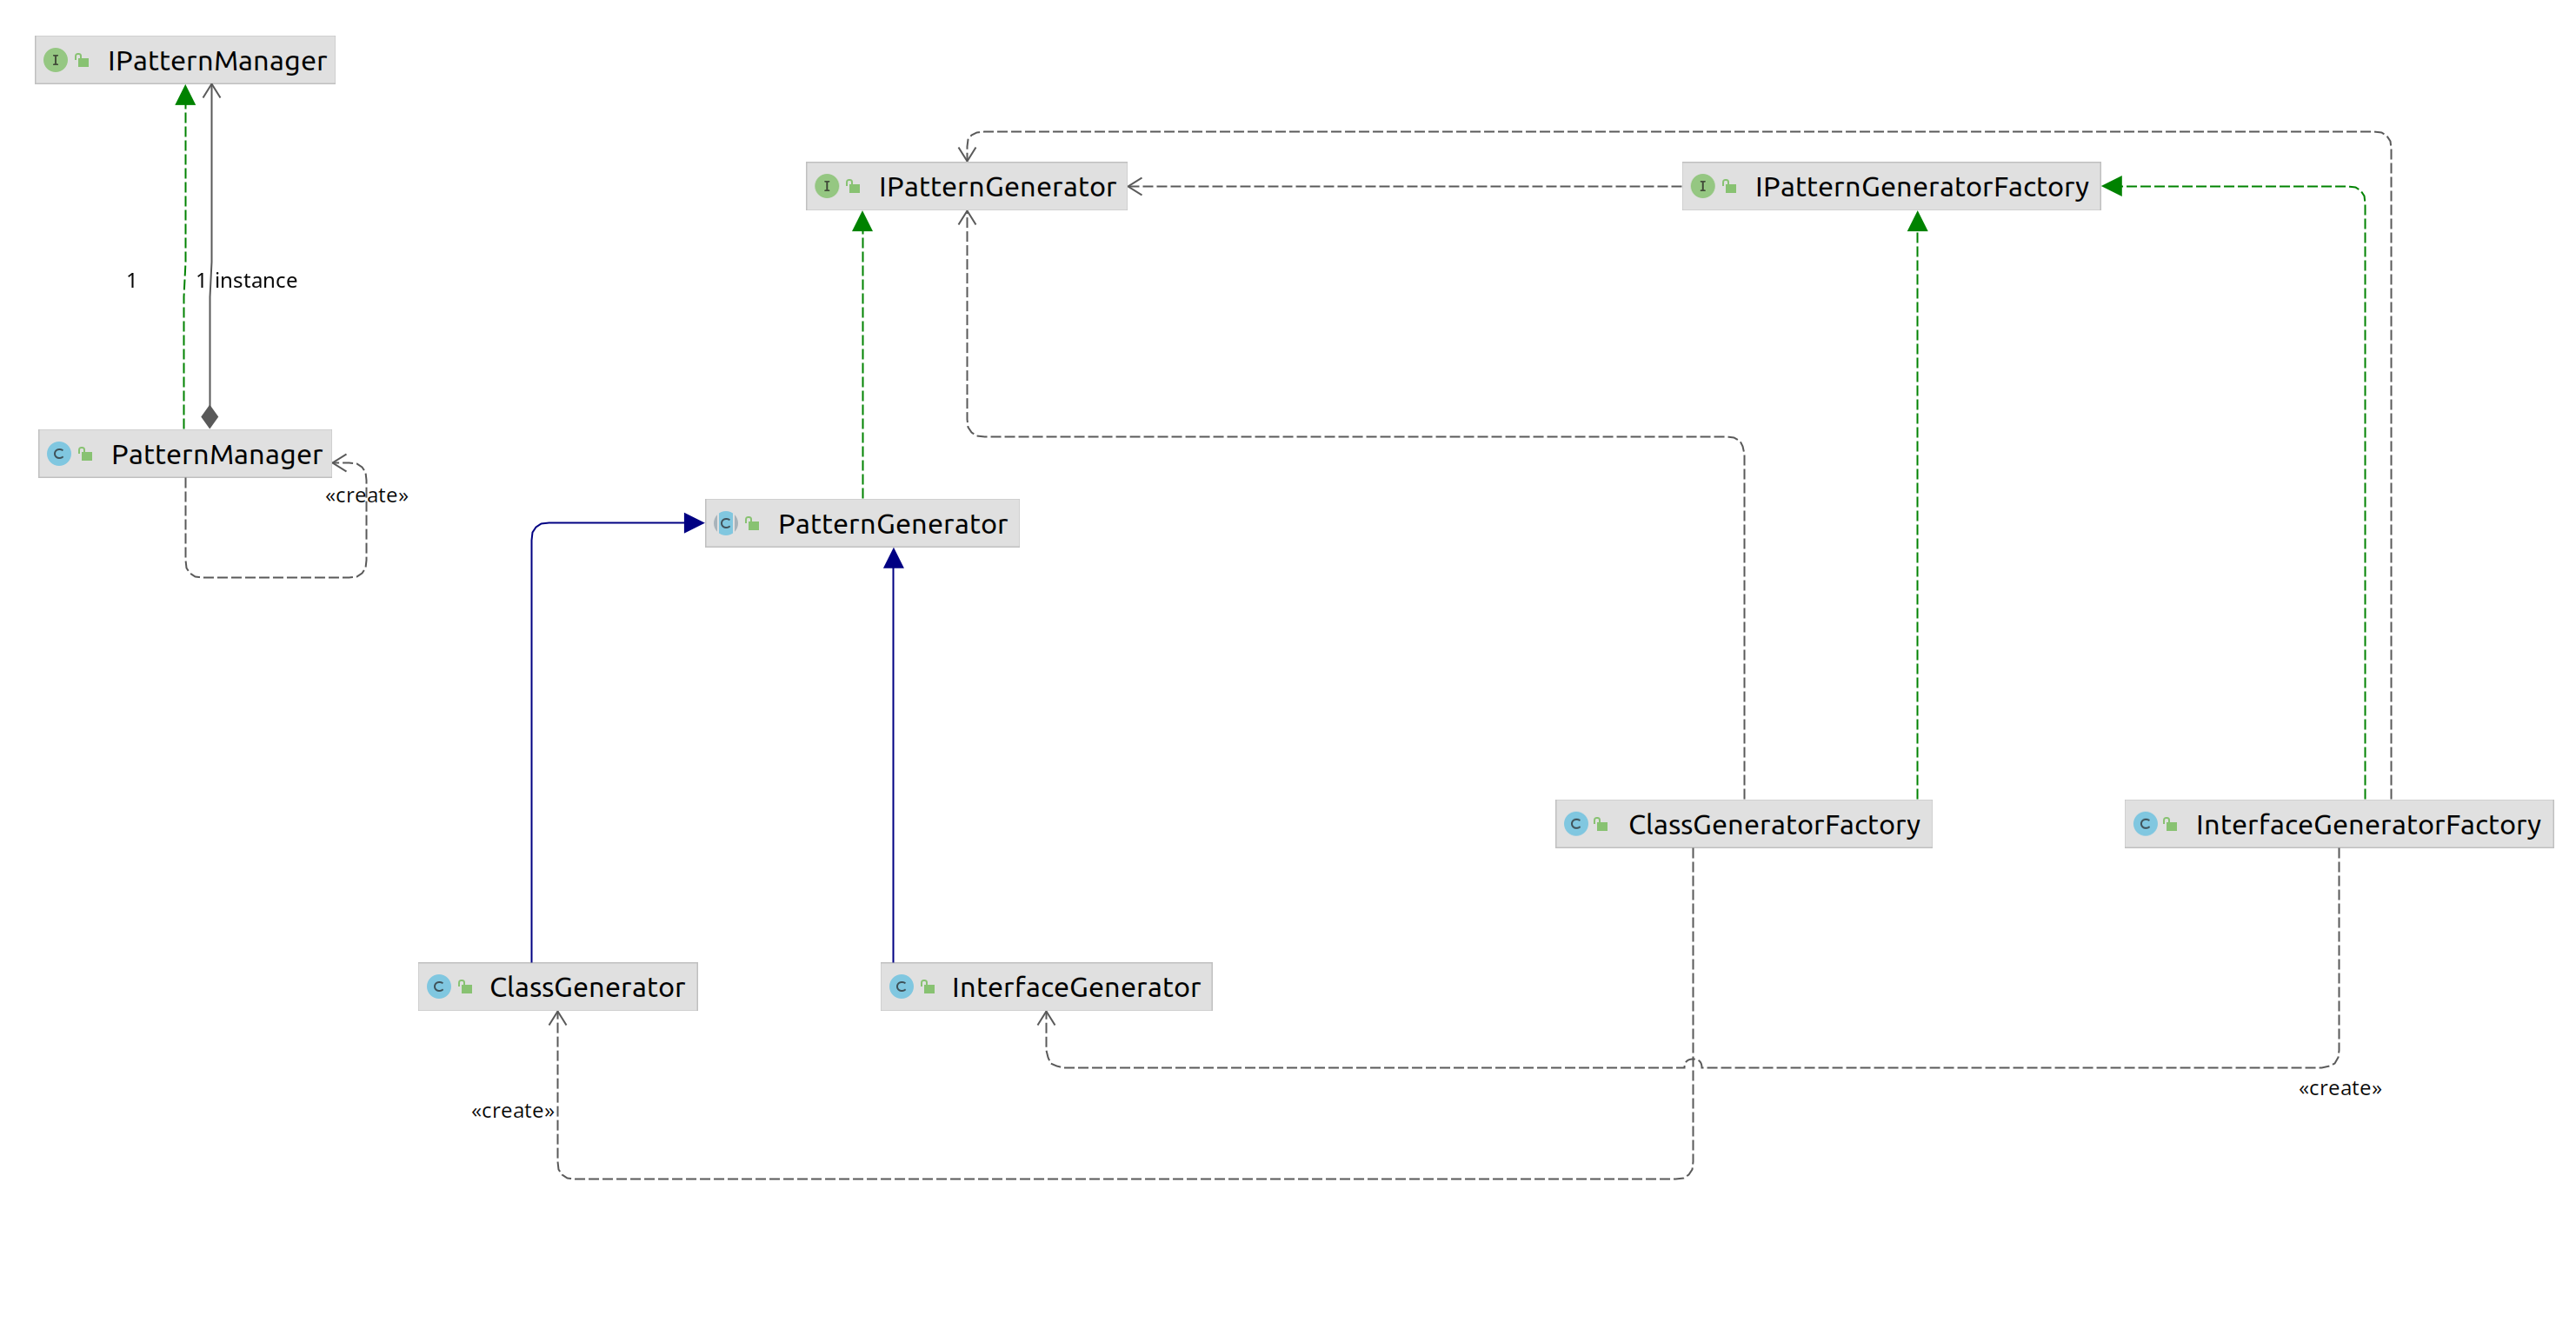
\includegraphics[width=1.0\textwidth]{Figures/controller.png}
    \caption{Διάγραμμα UML Πακέτου controller.}
    \label{fig:controllerUML}
\end{figure}
Το υποσύστημα του controller, είναι αρμόδιο για τις βασικές λειτουργίες του εργαλείου. Περιέχει την κλάση PatternManager, 
η οποία έχει ως σκοπό την παροχή των απαραίτητων πληροφοριών για κάποιο μοτίβο, καθώς και τα διαθέσιμα μοτίβα και κατηγορίες. 
Πιο συγκεκριμένα, δια μέσου αυτής της κλάσης η γραφική διεπαφή έχει διαθέσιμες τις δομές του πακέτου model, που 
περιγράφεται στην ενότητα \ref{sec:dpb.model}, δηλαδή, παρέχει ως πίνακες από Strings τις κατηγορίες και τα μοτίβα, τα οποία παίρνει 
από το υποσύστημα io της ενότητας \ref{sec:dpb.io}, και δημιουργεί αντικείμενα τύπου PatternClass αντλώντας το όνομα της κλάσης, 
την διεπαφή που υλοποιεί, τις μεθόδους και πεδία, καθώς και το εάν είναι αφηρημένη. Επίσης δημιουργεί αντικείμενα τύπου Method και Field, 
αντλώντας τις πληροφορίες από τον FileParser. Ακόμα, δημιουργεί και αντικείμενα τύπου PatternInterface, με όμοιο τρόπο, 
δηλαδή ανακτώντας το όνομα και τις μεθόδους από τον FileParser. Τέλος προσφέρει στο γραφικό περιβάλλον, μεθόδους για την σωστή ενημέρωση των ονομάτων.
\newline \newline
Στο υποσύστημα αυτό ανήκει και ιεραρχία κλάσεων για την δημιουργία των πηγαίων αρχείων java. δημιουργήσαμε αυτήν την ιεραρχία, καθώς,
ήταν απαραίτητο να εφαρμοστεί το μοτίβο Template Method \cite{GoF}, διότι η λειτουργία εξαγωγής των πηγαίων αρχείων χωρίστηκε σε κάποια βήματα, τα οποία είναι,
\begin{enumerate}
    \item Η προσθήκη του πακέτου που βρίσκεται η συγκεκριμένη κλάση ή διεπαφή του μοτίβου.
    \item Η προσθήκη των πεδίων μόνο στις κλάσεις. \label{enum:fields}
    \item Η προσθήκη των μεθόδων. \label{enum:methods}
    \item Η εξαγωγή του πηγαίου αρχείου που αφορά συγκεκριμένη κλάση ή διεπαφή του μοτίβου, με την χρήση του Eclipse API.
\end{enumerate}
Τα βήματα \ref{enum:fields} \& \ref{enum:methods}, είναι διαφορετικά για την περίπτωση που δημιουργούμε πηγαίο αρχείο κλάσης 
και διαφορετικό για την περίπτωση που δημιουργούμε πηγαίο αρχείο διεπαφής, καθώς οι διεπαφές δεν έχουν πεδία 
και οι μέθοδοι των διεπαφών δεν έχουν σώμα, Ακόμα διαφορά παρουσιάζει και ο ορισμός της διεπαφής και της κλάσης. 
Άρα κρίνεται απαραίτητη η χρήση του μοτίβου Template Method \cite{GoF}. Τέλος, η κλάση PatternGenerator, 
είναι υπεύθυνη και για την προσθήκη του πακέτου με τα annotations στο classpath του έργου του προγραμματιστή.
\newline \newline
Τέλος, για την μείωση της σύζευξης της ιεραρχίας IPatternGenerator με τα υπόλοιπα υποσυστήματα, 
χρησιμοποιήσαμε το μοτίβο Abstract Factory \cite{GoF}. Έτσι με αυτόν τον τρόπο τα υπόλοιπα υποσυστήματα, 
απλώς δημιουργούνε ένα \mbox{ClassGeneratorFactory} ή ένα \mbox{InterfaceGeneratorFactory}, 
και έτσι δημιουργούν έναν PatternGenerator ανάλογα την περίπτωση.
\section{dpb.io}
\label{sec:dpb.io}
\begin{figure}[H]
    \centering
    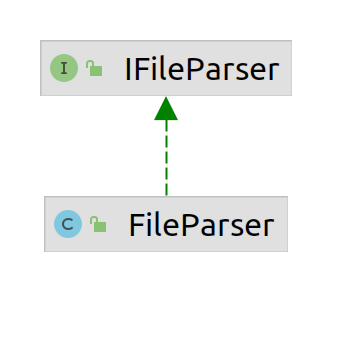
\includegraphics[width=1.0\textwidth]{Figures/io.png}
    \caption{Διάγραμμα UML Πακέτου io.}
    \label{fig:ioUML}
\end{figure}
Το υποσυστήματα αυτό, είναι το υποσύστημα που συνδέει το υπόλοιπο σύστημα με το αρχείο που περιγράφονται τα διάφορα μοτίβα. 
Η αρμοδιότητα του είναι αυτή ακριβώς, δηλαδή,  να διαβάζει το αρχείο xml και να μεταφέρει τις απαιτούμενες πληροφορίες στον controller. 
Αυτό που κάνει είναι να ανοίγει το αρχείο όπου περιγράφονται τα μοτίβα και να το διαβάζει. 
Είναι υπεύθυνο για την ανάκτηση των κατηγοριών και των μοτίβων, καθώς και την περιγραφή κάθε μοτίβου, 
επίσης διαβάζει και μεταβιβάζει με την μορφή συμβολοσειρών τα ονόματα των κλάσεων και διεπαφών, καθώς και τις ιδιότητες αυτών. Ακόμα, 
επιστρέφει το όνομα της διεπαφής που μπορεί να υλοποιεί μία κλάση, όπως, και το όνομα κάποιας κλάσης που μπορεί να επεκτείνει, 
και το αν μία κλάση είναι αφηρημένη. Επιστρέφει, το όνομα, την ορατότητα και τον επιστρεφόμενο τύπο, εάν είναι στατική η μέθοδος, 
όπως και τις παραμέτρους κάθε μεθόδου μίας διεπαφής ή κλάσης, επιπροσθέτως, εάν πρόκειται για κλάση επιστρέφει 
εάν η μέθοδος είναι αφηρημένη, καθώς και τον κώδικα που μπορεί να ορίζει κάποιο μοτίβο. Επιπλέον, 
διαβάζει το όνομα και τον τύπο κάθε πεδίου μίας κλάσης καθώς και εάν κάποιο πεδίο είναι στατικό.
Συμπληρωματικά, είναι υπεύθυνο, για την διαβίβαση κάποιων ιδιοτήτων των μοτίβων, όπως ποιες διεπαφές μπορεί 
να υλοποιεί κάποια νέα κλάση, καθώς και το εάν επιτρέπεται η προσθήκη νέας κλάσης και τέλος, τα annotations των νέων κλάσεων 
σύμφωνα με την διεπαφή που υλοποιούν. Τέλος, μεταβιβάζει στον controller και τα annotations που χαρακτηρίζουν μία κλάση ή διεπαφή του μοτίβου.
\section{dpb.model}
\label{sec:dpb.model}
\begin{figure}[H]
    \centering
    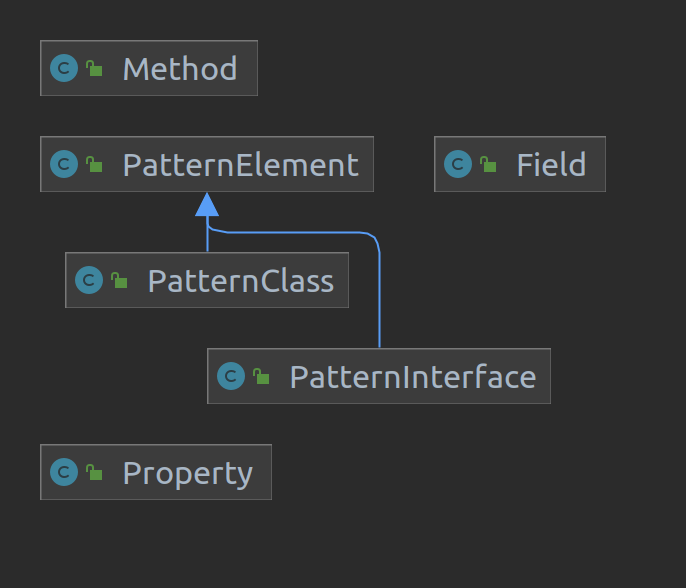
\includegraphics[width=1.0\textwidth]{Figures/model.png}
    \caption{Διάγραμμα UML Πακέτου model.}
    \label{fig:modelUML}
\end{figure}
Στο πακέτο αυτό, ορίζονται οι κλάσεις που αναπαριστούν τα αντικείμενα του πεδίου εφαρμογής.
\newline
Η κλάση Method αναπαριστά μία μέθοδο που ανήκει σε μία κλάση ή διεπαφή, έχει ως πεδία,
\begin{itemize}
    \item Το όνομα της μεθόδου.
    \item Τον επιστρεφόμενο τύπο της μεθόδου.
    \item Τον τροποποιητή της μεθόδου.
    \item Την λίστα των παραμέτρων της μεθόδου.
    \item Εάν είναι στατική μέθοδος.
    \item Εάν είναι αφηρημένη μέθοδος.
    \item Που ανήκει η μέθοδος.
    \item Τον κώδικα της μεθόδου.
    \item Εάν γίνεται Override η μέθοδος.
\end{itemize}
Ακόμα περιέχει getters \& setters και μία μέθοδο equal, για τον έλεγχο ισότητας με κάποιο άλλο αντικείμενο, 
καθώς χρειάζεται σε κάποιες περιπτώσεις.
\newline
Η κλάση Field αναπαριστά ένα πεδίο που ανήκει σε μία κλάση, έχει ως πεδία,
\begin{itemize}
    \item Το όνομα του πεδίου.
    \item Τον τύπο του πεδίου.
    \item Τον τροποποιητή του πεδίου.
    \item Εάν είναι στατικό πεδίο.
\end{itemize}
Αντίστοιχα και εδώ περιέχει getters \& setters και μία μέθοδο equal, για τον έλεγχο ισότητας με κάποιο άλλο αντικείμενο, 
καθώς χρειάζεται σε κάποιες περιπτώσεις.
\newline
Για την αναπαράσταση κλάσεων και διεπαφών, δημιουργήσαμε μία ιεραρχία, καθώς οι κλάσεις και οι διεπαφές 
έχουν πολλά κοινά χαρακτηριστικά, όπως, την κατηγορία μοτίβου και το μοτίβο που ανήκει μία κλάση/διεπαφή, το όνομα και την ορατότητα, 
καθώς και την λίστα με τις μεθόδους. Εκτός των κοινών χαρακτηριστικών έχουν και κάποιες διαφορές, για αυτόν τον λόγο προκύπτει η ανάγκη, 
να δημιουργήσουμε μία μαμά κλάση που θα έχει τα κοινά χαρακτηριστικά τους, και δύο κλάσεις που κληρονομούν την μαμά κλάση PatternElement, 
την κλάση PatternClass, η οποία αντιπροσωπεύει μία κλάση του μοτίβου και την PatternInterface που αντιπροσωπεύει μία διεπαφή του μοτίβου. 
Η κλάση PatternClass, περιέχει ως πεδία, την διεπαφή που υλοποιεί, την κλάση που επεκτείνει, εάν είναι αφηρημένη και 
μία λίστα με τα πεδία που έχει κάποια κλάση του μοτίβου. Ενώ η κλάση PatternInterface έχει ως μοναδικό 
πεδίο μία λίστα με τις κλάσεις που υλοποιούν την συγκεκριμένη διεπαφή, ώστε να μπορούμε να προσθέσουμε τις μεθόδους της 
διεπαφής στις κλάσεις που την υλοποιούν. Τέλοςμ εκτός από τις μεθόδους get \& set, έχουμε δημιουργήσει και μεθόδους 
οι οποίες προσθέτουν μία μέθοδο σε μία διεπαφή ή κλάση του μοτίβου, όπως και μεθόδους για την αφαίρεση κάποιας μεθόδου.
\newline
Τέλος, έμεινε η κλάση Property, η οποία απλώς αναπαριστά τις ιδιότητες κάθε μοτίβου που έχουμε παρουσιάσει παραπάνω. Η κλάση αυτή, 
έχει δύο πεδία, το ένα πεδίο αφορά το annotation που θα έχει κάποια καινούργια κλάση/διεπαφή που υλοποιεί/επεκτείνει, 
κάποια διεπαφή ή άλλη κλάση και το δεύτερο πεδίο αφορά την κλάση/διεπαφή που μπορεί να επεκτείνει/υλοποιεί η  νέα κλάση. Σαν μεθόδους έχει απλώς, 
getters \& setters.
